\documentclass[english,handout]{mlutalk}

\title{Reproducing Abstractive Text Summarization with Pretrained Encoders}
\subtitle{Data Mining, Winter Semester 2020/2021}
\author{Jan Heinrich Reimer}
\institute{Martin Luther University Halle-Wittenberg}
\date{March 30, 2021}
\titlegraphic{
\includegraphics[width=3cm]{figures/mlu-halle}}

\addbibresource{../literature/literature.bib}

\usepackage{tikz}
\usepackage{listings}
\usepackage{xspace}
\usepackage{biblatex}

\newcommand{\Elmo}{ELMo\xspace}
\newcommand{\Gpt}{GPT\xspace}
\newcommand{\Bert}{\textsc{Bert}\xspace}
\newcommand{\BertBase}{\textsc{Bert}-Base\xspace}
\newcommand{\BertTiny}{\textsc{Bert}-Tiny\xspace}
\newcommand{\BertSumExt}{\textsc{BertSumExt}\xspace}
\newcommand{\BertSumAbs}{\textsc{BertSumAbs}\xspace}
\newcommand{\TransformerAbs}{Transformer\textsc{Abs}\xspace}
\newcommand{\TransformerAbsTiny}{Transformer\textsc{Abs}Tiny\xspace}
\newcommand{\Rouge}{\mbox{ROUGE}\xspace}
\newcommand{\RougeN}[1]{\mbox{\Rouge-#1}\xspace}
\newcommand{\RougeL}{\mbox{\Rouge-L}\xspace}
\newcommand{\CnnDailyMail}{\mbox{CNN}/Daily Mail\xspace}
\newcommand{\WordPiece}{WordPiece\xspace}

\begin{document}

\titleframe

\begin{frame}{Abstractive Summarization}
    \begin{block}{Article}
        \scriptsize
        a university of iowa student has died nearly three months after a fall in rome in a suspected robbery attack in rome. andrew mogni, 20, from glen ellyn, illinois, had only just arrived for a semester program in italy when the incident happened in january. he was flown back to chicago via air ambulance on march 20, but he died on sunday. andrew mogni, 20, from glen ellyn, illinois, a university of iowa student has died nearly three months after a fall in rome in a suspected robbery he was taken to a medical 
        % facility in the chicago area, close to his family home in glen ellyn.he died on sunday at northwestern memorial hospital - medical examiner's office spokesman frank shuftan says a cause of death won't be released until monday at the earliest. initial police reports indicated the fall was an accident but authorities are investigating the possibility that mogni was robbed. on sunday, his cousin abby wrote online: `this morning my cousin andrew's soul was lifted up to heaven. initial police reports indicated the fall was an accident but authorities are investigating the possibility that mogni was robbed` at the beginning of january he went to rome to study aboard and on the way home from a party he was brutally attacked and thrown off a 40ft bridge and hit the concrete below. 
        \quad\(\cdots\)\quad
        % `he was in a coma and in critical condition for months.' paula barnett, who said she is a close family friend, told my suburban life, that mogni had only been in the country for six hours when the incident happened. she said he was was alone at the time of the alleged assault and personal items were stolen. she added that he was in a non-medically induced coma, having suffered serious infection and internal bleeding. mogni was a third-year
        finance major from glen ellyn, ill., who was participating in a semester-long program at john cabot university. mogni belonged to the school's chapter of the sigma nu fraternity, reports the chicago tribune who posted a sign outside a building reading `pray for mogni.' the fraternity's iowa chapter announced sunday afternoon via twitter that a memorial service will be held on campus to remember mogni.
    \end{block}
    \begin{block}{Summary}
        \scriptsize
        andrew mogni, 20, from glen ellyn, illinois, had only just arrived for a semester program when the incident happened in january. he was flown back to chicago via air on march 20 but he died on sunday. initial police reports indicated the fall was an accident but authorities are investigating the possibility that mogni was robbed. his cousin claims he was attacked and thrown 40ft from a bridge
    \end{block}
    \begin{itemize}
        \item too much text: condense to essential contents~\cite{Torres-Moreno2014}
        \item abstractive summarization more complex than extractive summ.
    \end{itemize}
\end{frame}

\begin{frame}{Automatic Summarization}
    \begin{itemize}
        \item program that takes long source text, outputs short summary
        \item often encoder-decoder architecture
        \begin{itemize}
            \item embed source text
            \item encode source text
            \item decode from internal representation
            \item gernerate/classify new words
        \end{itemize}
        \item similar to machine translation, but different length/vocabulary
        \item interpret each step as layer in deep neural network
    \end{itemize}
\end{frame}

\begin{frame}{\CnnDailyMail Datsasets~\cite{HermannKGEKSB2015}}
    \begin{itemize}
        \item longer news articles with short summary (see previous example)
        \item smaller datasets designed for benchmarking
        \item size: 240M~words
        \item limited training data for deep networks
    \end{itemize}
    \begin{block}{Idea}
        \begin{itemize}
            \item infer language context from pretrained encoders
            \item less task-specific training data needed
        \end{itemize}
    \end{block}
\end{frame}

\begin{frame}{\Bert for Summarization}
    \begin{itemize}
        \item use pretrained model like \Bert~\cite{DevlinCLT2019}
        \item \Bert already encodes language, pretrained on 3300M~words
        \item chosen variant: \BertBase
        \item only pretrained encoder, no decoder
    \end{itemize}
    \begin{block}{\BertSumAbs Model~\cite{LiuL2019}}
        \begin{enumerate}
            \item embed similar to \Bert embeddings
            \item encode embeddings with \BertBase
            \item decode \Bert representation using transformers~\cite{VaswaniSPUJGKP2017}
            \item generate new words
        \end{enumerate}
    \end{block}
\end{frame}

\begin{frame}{Preprocessing}
    \begin{itemize}
        \item download preprocessed datasets from replicated article~\cite{LiuL2019}
        \begin{itemize}
            \item sentences already split
            \item not truncated to 512~tokens, contrary to the author's claim \\ would discard 33\,\%~text on average
        \end{itemize}
        \item do not truncate, as it would delete important information
        \item split to sequence using \Bert \WordPiece tokenizer~\cite{DevlinCLT2019}
        \item map to vocabulary indices
    \end{itemize}
\end{frame}

\begin{frame}{Embeddings}
    \begin{itemize}
        \item learned word embeddings
        \begin{itemize}
            \item use \Bert vocabulary: 30K~token
            \item map to 2048-dimensional embeddings
        \end{itemize}
        \item learned position embeddings
        \begin{itemize}
            \item similar to \Bert embeddings
            \item extend maximum length to~4096, because articles are longer than \Bert's default max~512
        \end{itemize}
        \item 27M~parameters for embeddings, freshly trained
    \end{itemize}
\end{frame}

\begin{frame}{Encoder}
    \begin{itemize}
        \item encode embeddings with \BertBase~\cite{DevlinCLT2019}
        \item 12~transformer layers
        \item 768~hidden units of size~2048
        \item 85M~parameters for encoder, fine-tuned
    \end{itemize}
\end{frame}

\begin{frame}{Decoder~\cite{LiuL2019}}
    \begin{itemize}
        \item decode encoded embeddings with transformers~\cite{VaswaniSPUJGKP2017}
        \item similar to \BertBase hyperparameters
        \item 6~transformer layers
        \item 768~hidden units of size~2048
        \item dropout with probability~0.1
        \item 47M~parameters for encoder, freshly trained
    \end{itemize}
\end{frame}

\begin{frame}{Generator}
    \begin{itemize}
        \item map back embeddings to word probabilities
        \item simple linear layer with ReLU activation
        \item input size~2048
        \item output size~30K~(=vocabulary size)
        \item softmax to normalize probabilities
    \end{itemize}
\end{frame}

\begin{frame}{\BertSumAbs Takeaways}
    \begin{itemize}
        \item complex architecture
        \item 182M parameters
        \item some pretrained, others randomly initialized
    \end{itemize}
    \begin{block}{Alternative \TransformerAbsTiny model}
        \begin{itemize}
            \item smaller model for training on smaller machines
            \item 2~layers for encoder, 2~for decoder
            \item 8~hidden units
            \item 37K~parameters, freshly trained
            \item baseline for \BertSumAbs, based on \TransformerAbs~\cite{LiuL2019}
        \end{itemize}
    \end{block}
\end{frame}

\begin{frame}{Fine-tuning Schedule}
    \begin{itemize}
        \item train encoder and embeddings, decoder, generator seperately~\cite{LiuL2019}
        \item custom learning rates
        \item different warmup schedules
    \end{itemize}
    \begin{align*}
        \eta_E &= 2e^{-3} \cdot \min( \text{step}^{-0.5},\ \text{step} \cdot 20\,000^{-1.5} ) \\
        \eta_D &= 0.1 \cdot \min( \text{step}^{-0.5},\ \text{step} \cdot 10\,000^{-1.5} )
    \end{align*}
    \begin{itemize}
        \item decoder trained faster, encoder slower
        \item each iteration: take gradients for encoder parameters, take gradients for decoder parameters, update model with new parameters 
    \end{itemize}
\end{frame}

\begin{frame}{Training}
    \begin{itemize}
        \item training failed on available hardware
        \item \BertSumAbs trained on A100 GPU (40GB memory) \\ first 22\,500~steps recorded
        \item \TransformerAbsTiny trained on MX150 GPU (2GB memory) \\ first 200~steps recorded
        \item memory size overflows on both settings
    \end{itemize}
\end{frame}

\begin{frame}{Training Losses}
    \framesubtitle{\BertSumAbs}
    \begin{figure}
        \centering
        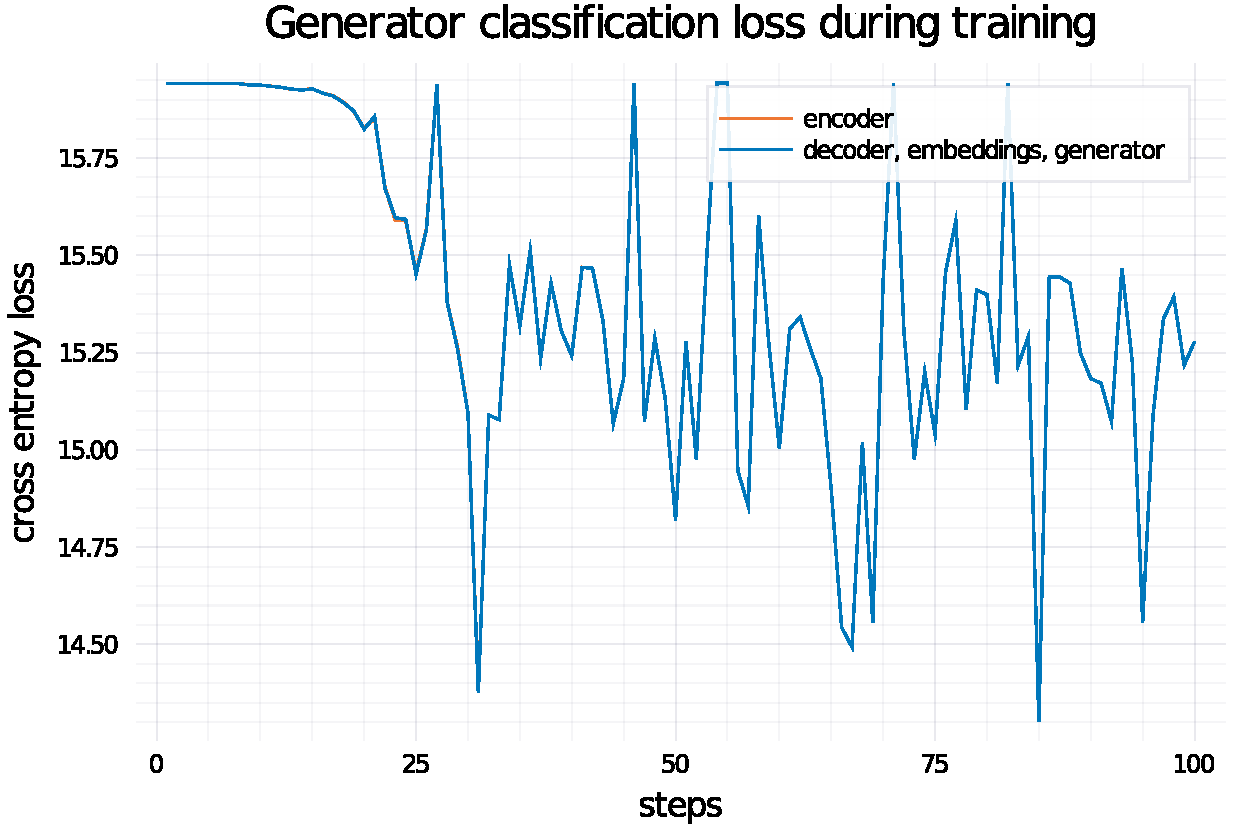
\includegraphics[width=0.6\linewidth]{figures/training-loss-bert-abs-100.pdf}
        \caption{Cross entropy loss for 100 training steps of \BertSumAbs}
    \end{figure}
    \begin{itemize}
        \item heavy oscillation after step~25
        \item oscillation continues to step~22\,500
    \end{itemize}
\end{frame}

\begin{frame}{Training Losses}
    \framesubtitle{\TransformerAbsTiny}
    \begin{figure}
        \centering
        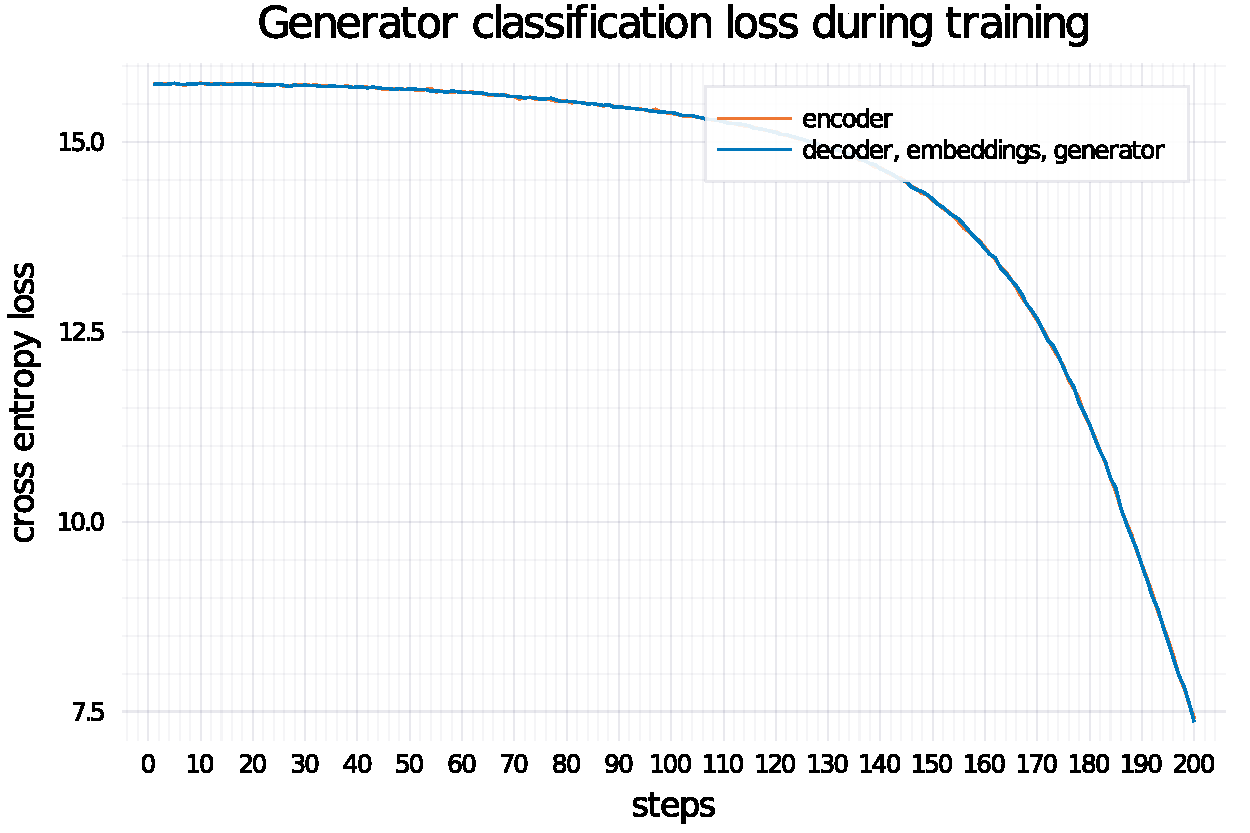
\includegraphics[width=0.6\linewidth]{figures/training-loss-transformer-abs-tiny.pdf}
        \caption{Cross entropy loss for 200 training steps of \TransformerAbsTiny}
    \end{figure}
    \begin{itemize}
        \item more stable decrease
    \end{itemize}
\end{frame}

\begin{frame}{Possible Causes for Failed Training}
    \begin{itemize}
        \item GPU memory too small to fit models and gradients
        \item model too complex, hard to differentiate
        \item training schedule leads to conflicting updates in the solution space
        \item reasons still unclear, difficult to debug
    \end{itemize}
\end{frame}

\begin{frame}[fragile]{Beam Search}
    \begin{itemize}
        \item decode token-by-token (shift outputs)
        \item keep track of the best \(n\) sequences
        \item possible sequences ranked by scoring function
        \item based on conditional probability for next token
        \item limit sequence length~\cite{WuSCLNMKCGMKSJL2016}, block redundance~\cite{PaulusXS2018}
        \item not used due to lacking a trained model
    \end{itemize}
\end{frame}

\begin{frame}{Quality Evaluation}
    \begin{block}{\Rouge scores~\cite{Lin2004}}
        \begin{itemize}
            \item automatic quality evaluation
            \item \RougeN{1}/\RougeN{2} metric for measuring informativeness 
            \item \RougeL for measuring fluency
        \end{itemize}
    \end{block}
    \begin{block}{Manual evaluation}
        \begin{itemize}
            \item human assessment
            \item labels from 0~(unreadable, unrelated) to 2~(informative, fluent, non-repetitive)
        \end{itemize}
    \end{block}
    \begin{itemize}
        \item not conducted due to lacking a trained model
    \end{itemize}
\end{frame}

\begin{frame}{Conclusion}
    \begin{itemize}
        \item unable to reproduce results
        \item difficulties in training
        \item no model fully trained 
        \item concerning model size, possibly oversized
        \item high computational cost not worth it for minor improvements
    \end{itemize}
        
\end{frame}

\begin{frame}{Future Work}
    \begin{itemize}
        \item train \BertSumAbs model with smaller \Bert variants, \\ e.g., \BertTiny~\cite{TurcCLT2019}
        \item model compression
        \item model regularization
        \item other language models might be better suited, \\ e.g., GPT-3~\cite{BrownMRSKDNSSAA2020} with few-shot learning
    \end{itemize}
    \thankyou
\end{frame}

% \begin{frame}{XXXXXXX}
% \end{frame}

% \begin{frame}{XXXXXXX}
% \end{frame}

\appendix
\section{\appendixname}

\bibliographyframe

\end{document}


